
\documentclass{beamer}

\mode<presentation> 
  {
  \usetheme{Madrid}
  }

%%%%%%%%%%%%%%%%%%%%%%%%%%%%%%%%%%%%% PAQUETES %%%%%%%%%%%%%%%%%%%%%%%%%%%%%%%%%%%%%%%%%%

\usepackage[utf8]{inputenc}
\usepackage[spanish]{babel}
\usepackage[T1]{fontenc}
\usepackage{graphicx}
\usepackage{booktabs} % Allows the use of \toprule, \midrule and \bottomrule in tables
\usepackage{animate} % para crear el gif de kmeans
%\usepackage[usenames, dvipsnames]{xcolor} % para los colores
\usepackage{listings} % para el codigo fuente
\lstset
  {
  %backgroundcolor=\color{},   % Indica el color de fondo
  basicstyle=\footnotesize,
  commentstyle=\color{green},      % Estilo de los comentarios
  }
\usepackage{hyperref} % para las referencias cruzadas
%TODO revisar
\hypersetup
{
    %bookmarks=true,         % show bookmarks bar?
    %unicode=false,          % non-Latin characters in Acrobat’s bookmarks
    %pdftoolbar=true,        % show Acrobat’s toolbar?
    %pdfmenubar=true,        % show Acrobat’s menu?
    %pdffitwindow=false,     % window fit to page when opened
    pdfstartview={Fit},    % fits the width of the page to the window
    pdftitle={Estudio comparativo de Algoritmos de machine learning e implementación en Hadoop},    % title
    pdfauthor={David Retana Ribeiro},     % author
    pdfsubject={Big data y machine learning},   % subject of the document
    pdfkeywords={computacion paralela, apache hadoop, apache spark, machine Learning, big data, python, k means,
               naive bayes, yarn, hdfs, cluster}, % list of keywords
    pdfnewwindow=true,      % links in new PDF window
    %colorlinks=true,       % false: boxed links; true: colored links
    %linkcolor=red,          % color of internal links (change box color with linkbordercolor)
    %citecolor=green,        % color of links to bibliography
    %filecolor=magenta,      % color of file links
    %urlcolor=cyan           % color of external links
}

%%%%%%%%%%%%%%%%%%%%%%%%%%%%%%%%%%%%%% TITULO %%%%%%%%%%%%%%%%%%%%%%%%%%%%%%%%%%%%%%%%%%%

\title[Machine Learning y Big Data]
      {Estudio comparativo de algoritmos paralelos de machine learning e implementación en Hadoop}
\author{David Retana Ribeiro}
\institute[UCM]{Universidad Complutense de Madrid \\ \medskip \texttt{davidret@ucm.es}}
\date{4 de Octubre de 2017}

%%%%%%%%%%%%%%%%%%%%%%%%%%%%%%%%%%%%%%%%%%%%%%%%%%%%%%%%%%%%%%%%%%%%%%%%%%%%%%%%%%%%%%%%%

\begin{document}

%%%%%%%%%%%%%%%%%%%%%%%%%%%%%%%%%%%%%%%%%%%%%%%%%%%%%%%%%%%%%%%%%%%%%%%%%%%%%%%%%%%%%%%%%

\begin{frame} % Portada
\titlepage
\end{frame}

%%%%%%%%%%%%%%%%%%%%%%%%%%%%%%%%%%%%%%%%%%%%%%%%%%%%%%%%%%%%%%%%%%%%%%%%%%%%%%%%%%%%%%%%%%

\begin{frame} % Indice de contenidos
\frametitle{Índice de contenidos}
\tableofcontents
\end{frame}

%%%%%%%%%%%%%%%%%%%%%%%%%%%%%%%%%%%%%%%%%%%%%%%%%%%%%%%%%%%%%%%%%%%%%%%%%%%%%%%%%%%%%%%%%%
%%%%%%%%%%%%%%%%%%%%%%%%%%%%%%%%%%%% INTRODUCCION %%%%%%%%%%%%%%%%%%%%%%%%%%%%%%%%%%%%%%%%
%%%%%%%%%%%%%%%%%%%%%%%%%%%%%%%%%%%%%%%%%%%%%%%%%%%%%%%%%%%%%%%%%%%%%%%%%%%%%%%%%%%%%%%%%%

\section{Introducción}

\begin{frame} % Introduccion a Big data y machine learning
  \frametitle{Introducción}
  \begin{block}{Big Data}
  Vivimos en la era de los datos, cada día se producen más y más datos  que necesitan ser almacenados y
  procesados para poder sacarles partido.\\
  El termino \textbf{Big Data} nace como un concepto para hacer referencia a la incapacidad de 
  los sistemas tradicionales de almacenar y procesar un conjunto masivo de datos.
  \end{block}
  
  \begin{block}{Machine Learning}
  El \textbf{machine learning} es una rama de la inteligencia artificial que permite crear sistemas que 
  aprendan automáticamente sin ser programados explícitamente para ello.\\
  Consiste en sacar patrones de los datos con el fin de crear modelos que permitan obtener un beneficio
  de los mismos. Estos modelos se apoyan en fórmulas matemáticas para su creación, principalmente de 
  álgebra lineal y estadística.
  \end{block}
\end{frame}

%%%%%%%%%%%%%%%%%%%%%%%%%%%%%%%%%%%%%%%%%%%%%%%%%%%%%%%%%%%%%%%%%%%%%%%%%%%%%%%%%%%%%%%%%%

\begin{frame} % Como encajan Hadoop, mapreduce, spark y machine learning al big data
  \frametitle{Apache Hadoop y Apache Spark}
  Actualmente, existen diversas herramientas que nos permiten trabajar con las grandes cantidades de datos
  manejadas en el \textit{Big Data}. \textit{Apache Hadoop} es el software base que nos permite desplegar
  un cluster de máquinas sobre el que trabajar y desarrollar nuestros algoritmos.\\
  Hadoop incluye MapReduce como motor de procesamiento por defecto pero también es perfectamente compatible con Spark.
  
\includegraphics[width=0.5\textwidth]{C:/Users/David/Desktop/TFG/TFGLatex/presentacion/recursos/hadoop_logo.png}%
  
\includegraphics[width=0.5\textwidth]{C:/Users/David/Desktop/TFG/TFGLatex/presentacion/recursos/spark_logo.png}
\end{frame}

%%%%%%%%%%%%%%%%%%%%%%%%%%%%%%%%%%%%%%%%%%%%%%%%%%%%%%%%%%%%%%%%%%%%%%%%%%%%%%%%%%%%%%%%%%
%%%%%%%%%%%%%%%%%%%%%%%%%%%%%%%% DESPLIEGUE HADOOP %%%%%%%%%%%%%%%%%%%%%%%%%%%%%%%%%%%%%%%
%%%%%%%%%%%%%%%%%%%%%%%%%%%%%%%%%%%%%%%%%%%%%%%%%%%%%%%%%%%%%%%%%%%%%%%%%%%%%%%%%%%%%%%%%%
\section{Despliegue de un \textit{cluster Hadoop}}

\begin{frame} % imagen de topologia de un cluster Hadoop
\frametitle{Topología de un cluster Hadoop}
\begin{figure}
\centering
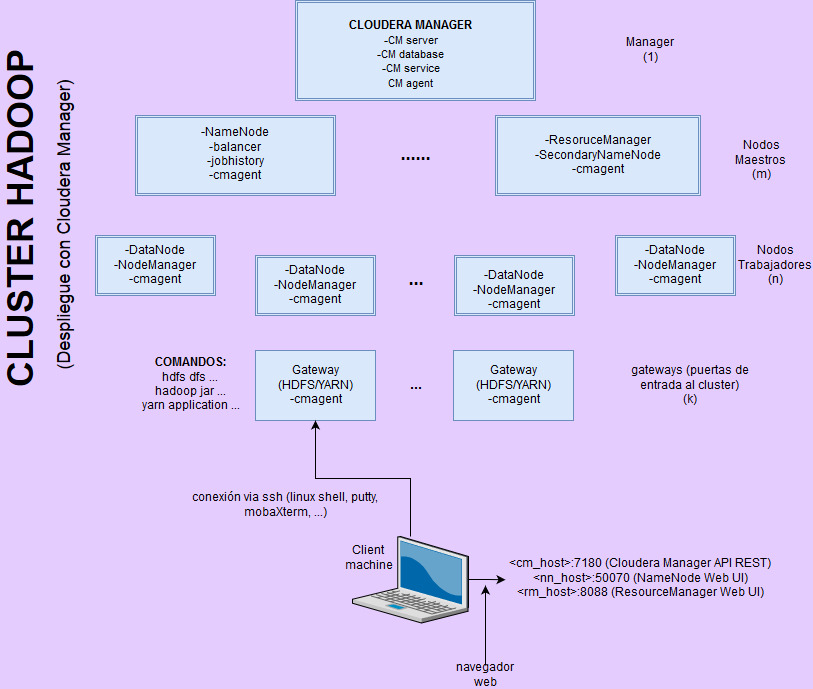
\includegraphics[scale=0.3]{C:/Users/David/Desktop/TFG/TFGLatex/imagenes/hadoop_topology.jpg}
\end{figure}
\end{frame}

%%%%%%%%%%%%%%%%%%%%%%%%%%%%%%%%%%%%%%%%%%%%%%%%%%%%%%%%%%%%%%%%%%%%%%%%%%%%%%%%%%%%%%%%%%

\subsection{\textit{HDFS} y \textit{YARN}}

\begin{frame}[fragile] % fragile permite añadir codigo con lstlisting
\frametitle{HDFS}
\begin{block}{Hadoop Distributed File System}
Ejemplos de comandos de HDFS:
\begin{lstlisting}[language=bash, numbers=none, frame=single]
$ # crea un directorio recursivamente
$ hdfs dfs -mkdir -R <direccion_a_crear>
$ # sube un archivo de local a HDFS
$ hdfs dfs -put <path_archivo_local> <path_hdfs> 
$ # Descarga un archivo de HDFS a local
$ hdfs dfs -get <path_hdfs> <path_local> 
\end{lstlisting}

En un navegador escribimos: \path{<ip_namenode>:50070}

\end{block}
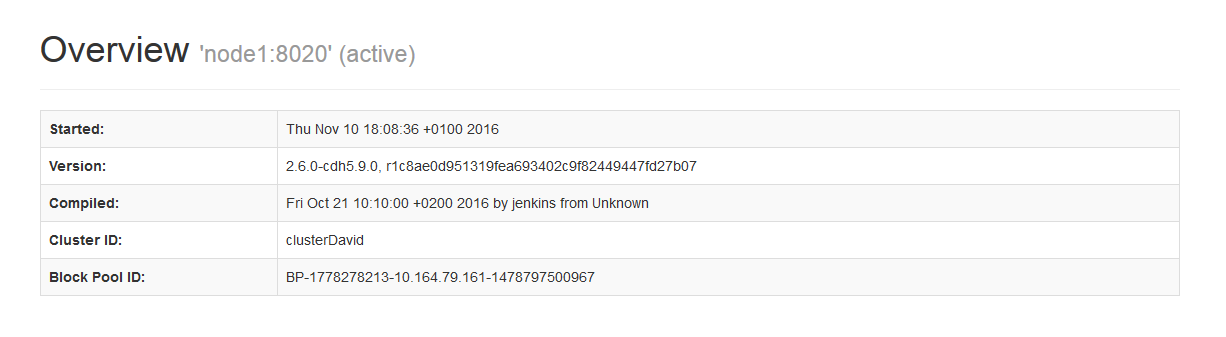
\includegraphics[width=0.9\textwidth]{C:/Users/David/Desktop/TFG/TFGLatex/presentacion/recursos/overview_cluster.png}
\end{frame}

%%%%%%%%%%%%%%%%%%%%%%%%%%%%%%%%%%%%%%%%%%%%%%%%%%%%%%%%%%%%%%%%%%%%%%%%%%%%%%%%%%%%%%%%%%

\begin{frame}[fragile]
  \frametitle{YARN v2 (\textit{MapReduce} incluido)}
  Lanzamiento de un trabajo \textit{MapReduce} en un \textit{cluster Hadoop}
  \begin{lstlisting}[language=bash, numbers=none, frame=single]
$ hadoop jar WordCount.jar WordCount \
  <input_path> <output_path>
  \end{lstlisting}
  
  En un navegador escribimos: \path{<ip_resource_manager>:8088}\\
  De esta manera podemos ver los trabajos que están corriendo en nuestro \textit{cluster} y su progreso.
  
  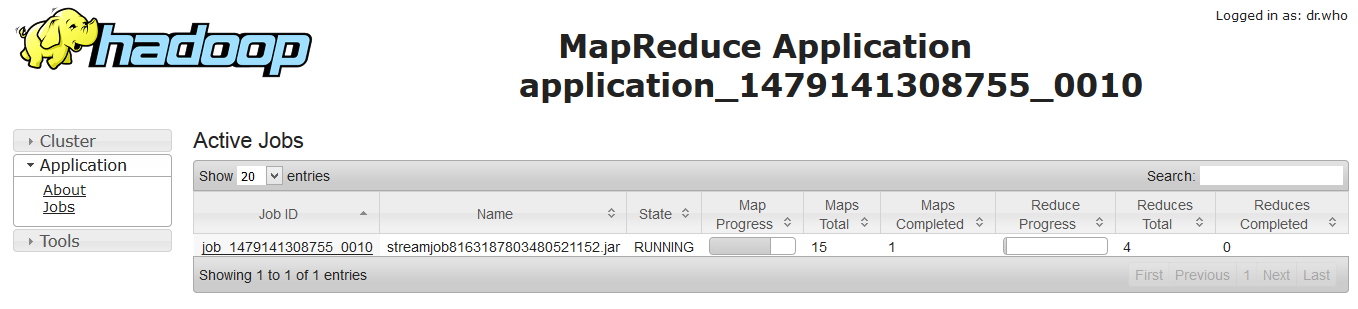
\includegraphics[width=\textwidth]{C:/Users/David/Desktop/TFG/TFGLatex/presentacion/recursos/mapreduce_application.png}
  
\end{frame}

%%%%%%%%%%%%%%%%%%%%%%%%%%%%%%%%%%%%%%%%%%%%%%%%%%%%%%%%%%%%%%%%%%%%%%%%%%%%%%%%%%%%%%%%%%
\subsection{\textit{Spark}}

\begin{frame}[fragile]
\frametitle{\textit{Apache Spark}}

\begin{block}{}
\begin{lstlisting}[language=bash, numbers=none, frame=single]
$ pyspark --master yarn-client
\end{lstlisting}
\end{block}

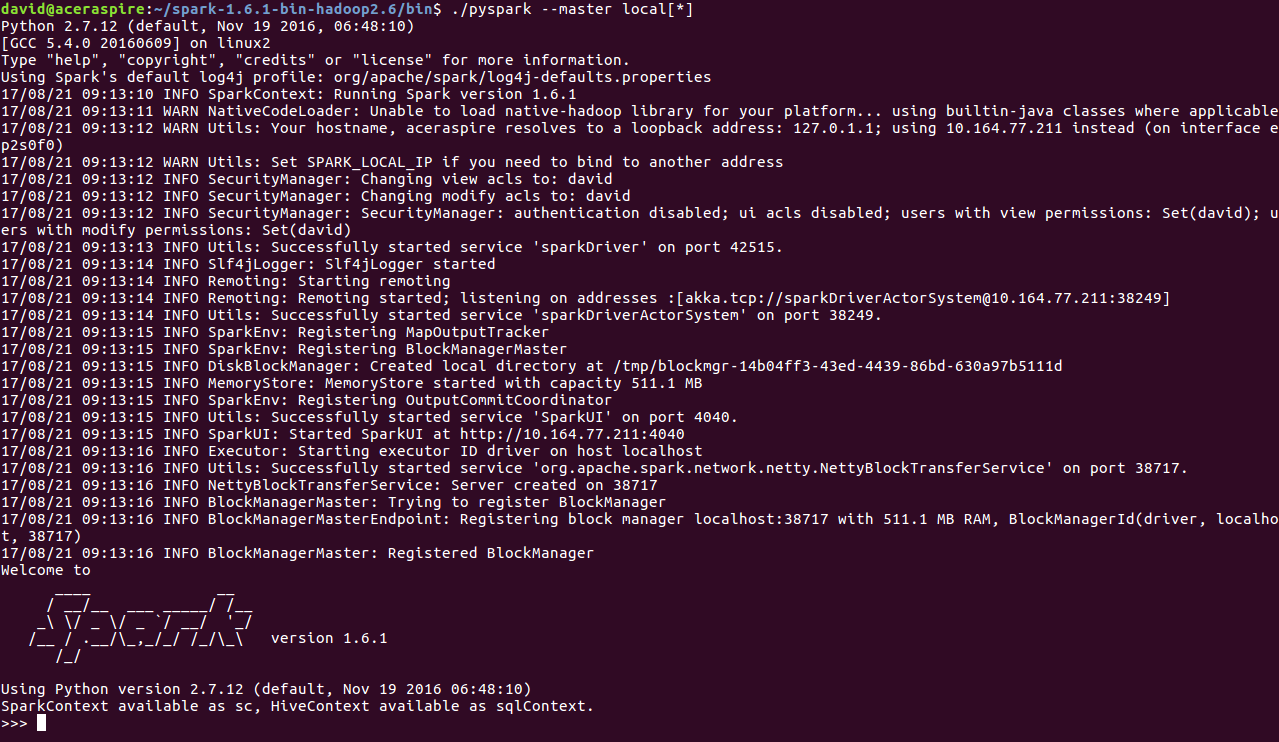
\includegraphics[width=\textwidth]{C:/Users/David/Desktop/TFG/TFGLatex/presentacion/recursos/pyspark_shell.png}

\begin{block}{}
\begin{lstlisting}[language=bash, numbers=none, frame=single, showstringspaces=false]
>>> rdd = sc.parallelize(range(1000))
>>> n = rdd.count()
>>> print("Numero de elementos: ", n)
\end{lstlisting}
\end{block}

\end{frame}

%%%%%%%%%%%%%%%%%%%%%%%%%%%%%%%%%%%%%%%%%%%%%%%%%%%%%%%%%%%%%%%%%%%%%%%%%%%%%%%%%%%%%%%%%%

\begin{frame}
  \frametitle{Cloudera Manager}
  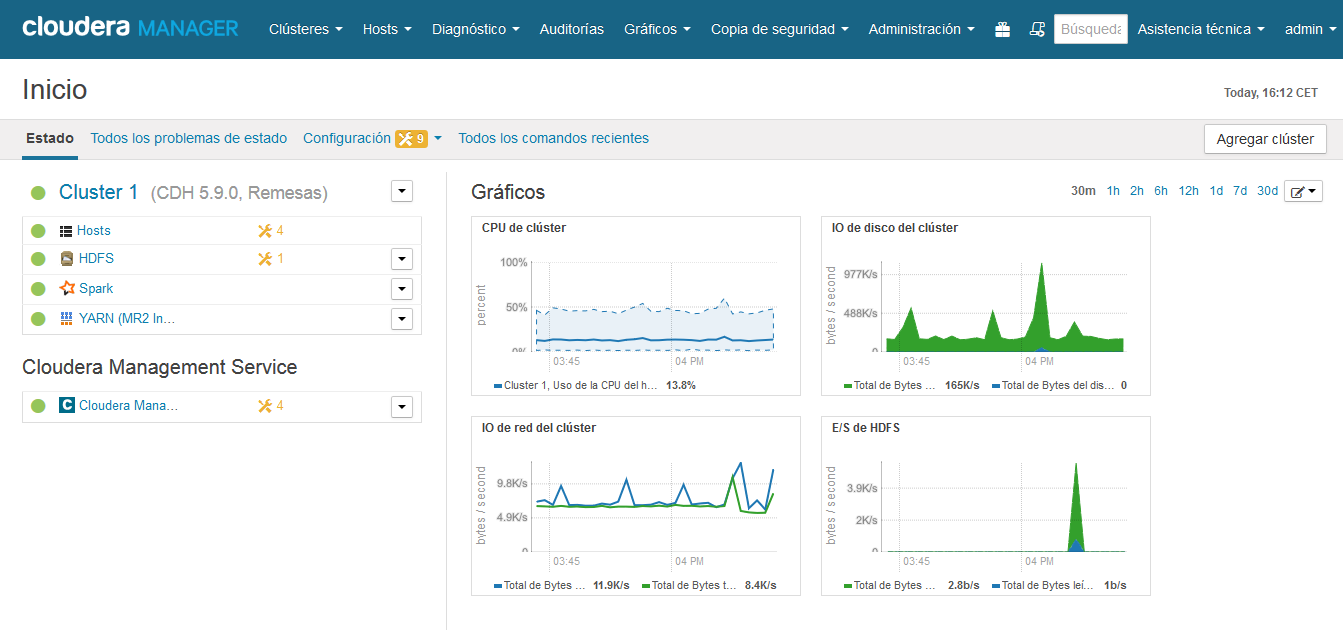
\includegraphics[width=\textwidth]{C:/Users/David/Desktop/TFG/TFGLatex/presentacion/recursos/cloudera_manager.png}
\end{frame}

%%%%%%%%%%%%%%%%%%%%%%%%%%%%%%%%%%%%%%%%%%%%%%%%%%%%%%%%%%%%%%%%%%%%%%%%%%%%%%%%%%%%%%%%%%
%%%%%%%%%%%%%%%%%%%%%%%%%%%%%%%%% MACHINE LEARNING %%%%%%%%%%%%%%%%%%%%%%%%%%%%%%%%%%%%%%%
%%%%%%%%%%%%%%%%%%%%%%%%%%%%%%%%%%%%%%%%%%%%%%%%%%%%%%%%%%%%%%%%%%%%%%%%%%%%%%%%%%%%%%%%%%
\section{\textit{Machine Learning}}

%El desarrollo de algoritmos paralelos de machine learning, debido a su carácter experimental,
%necesitan ser entrenados varias veces para obtener el mejor ajuste de los parámetros. De esta manera, el cómputo
%paralelo se vuelve fundamental para reducir los tiempos de ejecución.
\begin{frame} % machine learning en general
\frametitle{Machine Learning}
¿Cómo encaja el machine learning en el Big Data?
\centering
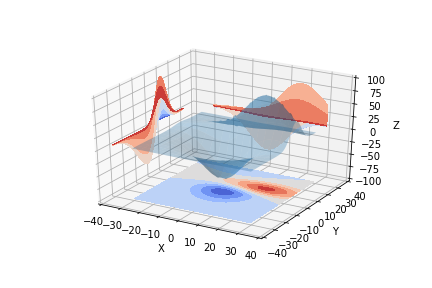
\includegraphics[scale=0.5]{C:/Users/David/Desktop/TFG/TFGLatex/presentacion/recursos/contour_surface.png}
Debido a que el Machine Learning se alimenta de los datos, cuantos más datos tengamos para entrenar los modelos más 
preciosos serán estos, por lo que los términos Big Data y Machine Learning están estrechamente relacionados.
\end{frame}

%%%%%%%%%%%%%%%%%%%%%%%%%%%%%%%%%%%%%%%%%%%%%%%%%%%%%%%%%%%%%%%%%%%%%%%%%%%%%%%%%%%%%%%%%%

\subsection{Algoritmo de \textit{K-Means}}

\begin{frame}[fragile] % contar aprendizaje no supervisado y algoritmo kmeans por encima
\frametitle{Algoritmo de K-Means}
En el aprendizaje no supervisado es el propio algoritmo el que debe encontrar los patrones ocultos entre los datos.
El algoritmo de K-Means es un algoritmo muy popular de clusterización que se encaja dentro de esta categoría de 
aprendizaje no supervisado.\\
Veamos de una manera gráfica su funcionamiento
\end{frame}

%%%%%%%%%%%%%%%%%%%%%%%%%%%%%%%%%%%%%%%%%%%%%%%%%%%%%%%%%%%%%%%%%%%%%%%%%%%%%%%%%%%%%%%%%%

\begin{frame} % kmeans gif
  \animategraphics[loop, controls, width=\linewidth]{1} % {n} cuanto menor mas lento
  {C:/Users/David/Desktop/TFG/TFGLatex/presentacion/recursos/kmeans_imagen}{0}{4}
\end{frame}

%%%%%%%%%%%%%%%%%%%%%%%%%%%%%%%%%%%%%%%%%%%%%%%%%%%%%%%%%%%%%%%%%%%%%%%%%%%%%%%%%%%%%%%%%%

%TODO revisar
\begin{frame}[fragile] % exponer el codigo fuente (explicar porqué se usa spark en vez de MapReduce)
\frametitle{Código fuente}
%\lstinputlisting[caption=KMeansSpark.py, language=Python, firstline=8, lastline=72]
%                {C:/Users/David/Desktop/TFG/implementaciones/KMeansSpark.py}
\end{frame}

%%%%%%%%%%%%%%%%%%%%%%%%%%%%%%%%%%%%%%%%%%%%%%%%%%%%%%%%%%%%%%%%%%%%%%%%%%%%%%%%%%%%%%%%%%

\begin{frame} % tabla y grafica comparativa de tiempos (spark vs numpy)
\frametitle{Comparativa de rendimiento}

\end{frame}

%%%%%%%%%%%%%%%%%%%%%%%%%%%%%%%%%%%%%%%%%%%%%%%%%%%%%%%%%%%%%%%%%%%%%%%%%%%%%%%%%%%%%%%%%%

\begin{frame}
\Huge{\centerline{Fin}}
\end{frame}

%%%%%%%%%%%%%%%%%%%%%%%%%%%%%%%%%%%%%%%%%%%%%%%%%%%%%%%%%%%%%%%%%%%%%%%%%%%%%%%%%%%%%%%%%%

\end{document} 